\documentclass[UTF8, a4paper]{ctexart}
\usepackage[margin=1in]{geometry} % 页边距调整
\usepackage{ctex}
\usepackage{array, amsmath, amssymb}

\usepackage{booktabs, tabularx, multirow, multicol} % 表格拓展支持
\usepackage{graphicx, subfigure, float} % 图片排版支持

\usepackage{algorithm, algpseudocode} % 伪代码支持
\renewcommand{\algorithmicrequire}{\textbf{Input:}}  
\renewcommand{\algorithmicensure}{\textbf{Output:}} 

\usepackage{tikz, mathpazo} % 基本绘图支持
\usepackage{flowchart} % 流程图支持
\usepackage{pgf-umlcd} % UML类图支持
\usetikzlibrary{arrows, shapes, chains, shapes.geometric}

\usepackage{listings} % 代码块支持
\usepackage{xcolor}
\lstset{
	language		= c++,
	backgroundcolor	= \color{white},
	basicstyle		= \footnotesize\ttfamily,
	keywordstyle	= \color{blue},
	stringstyle		= \color{red!58!blue!82}\ttfamily,
	commentstyle	= \color{darkgray},
	rulesepcolor	= \color{red!20!green!20!blue!20},
	columns			= fullflexible,
	breaklines		= true,
	captionpos		= b,
	tabsize			= 4,
	frame			= single,
	escapeinside	= {\%*}{*)}
}
%%示例
% \begin{lstlisting}[caption={}]
% #include <iostream>
% int main(int argc, char *argv[]) {
% 	std::cout << "Hello World!" << std::endl;
% 	return 0;
% }
% \end{lstlisting}

\usepackage{datetime} %日期
\renewcommand{\today}{\number\year{年}\number\month{月}\number\day{日}}

\begin{document}

\begin{center}
	\zihao{3}《数据结构》实验报告
\end{center}
\zihao{5}

\newcolumntype{Y}{>{\raggedleft\arraybackslash}X}
\noindent\begin{tabularx}{\textwidth}{XcY}
	  {班 级:}\;\underline{DL062123}
	& {姓 名:}\;\underline{项乔栋}
	& {学 号:}\;\underline{2021302468} \\
	  {邮 箱:}\;\underline{13282135976@sina.cn}
	& {日 期:}\;\underline{\today}
	& {编 号:}\;\underline{DS07}
\end{tabularx}
~\\

\noindent\textbf{$\circledcirc$
实验题目:\quad{哈夫曼编/译码器}} \par
\noindent\textbf{$\circledcirc$
实验目的:\quad{从哈夫曼编码树实践对树结构的应用}} \par
\noindent\textbf{$\circledcirc$
实验内容:\quad{哈夫曼编/译码器的实现}} \par

\subsection*{一、需求分析}
\noindent\fbox{
\begin{tabularx}{\textwidth}{lY}
\bf{Description}
& \parbox[t]{\linewidth}{
	写一个哈夫曼码的编/译码系统,要求能够对要传输的报文进行编码和解码。
	构造哈夫曼树时,权值小的放左子树,权值大的放右子树,编码时右子树编码为1,左子树编码为0。
} \\

\bf{Input}
& \parbox[t]{\linewidth}{
	输入表示字符集大小为n(n$\leq$100)的正整数,以及n个字符和n个权值(正整数,值越大表示该字符出现的概率越大);
	输入串长小于或等于100的目标报文。
} \\

\bf{Output}
& \parbox[t]{\linewidth}{
	经过编码后的二进制码,占一行;
	以及对应解码后的报文,占一行;
	最后输出一个回车符
} \\

\bf{Sample Input}
& \fbox{\parbox[t]{\linewidth}{\bf{
	\mbox{5} \\
	\mbox{a b c d e} \\
	\mbox{12 40 15 8 25} \\
	\mbox{bbbaddeccbbb}
}}} \\

\bf{Sample Output}
& \fbox{\parbox[t]{\linewidth}{\bf{
	\mbox{00011111110111010110110000} \\
	\mbox{bbbaddeccbbb}
}}}
\end{tabularx}}

\subsection*{二、概要设计}
% 摘要
\par
1.\;基本操作: \par
	CreateFromIO() $\rightarrow$ HuffmanTree \par
	\qquad\textbf{操作结果:}\;从IO流创建哈夫曼编码树 \par
	Build(items:Array<Pair<String,Integer>{>}) $\rightarrow$ HuffmanTree \par
	\qquad\textbf{操作结果:}\;从元单词权值列表创建哈夫曼编码树 \par
	EncodeWord(word:String,encoder:HuffmanTree) $\rightarrow$ String \par
	\qquad\textbf{操作结果:}\;获取给定哈夫曼编码下元单词的编码 \par
	Encode(text:String,encoder:HuffmanTree) $\rightarrow$ String \par
	\qquad\textbf{操作结果:}\;获取给定哈夫曼编码下文本的编码文本 \par
	DecodeSingle(code:String,decoder:HuffmanTree) $\rightarrow$ String \par
	\qquad\textbf{操作结果:}\;获取给定哈夫曼编码下元编码的译码单词 \par
	Decode(encoded\_text:String,decoder:HuffmanTree) $\rightarrow$ String \par
	\qquad\textbf{操作结果:}\;获取给定哈夫曼编码下编码的译码文本 \par
2.\;程序模块: \par
1) 主程序 \par
2) IO支持 \par
3) 哈夫曼树构建 \par
4) 哈夫曼编码模块 \par
5) 哈夫曼译码模块 \par
\begin{figure}[H]
	\begin{minipage}[t]{\linewidth}
		\centering
		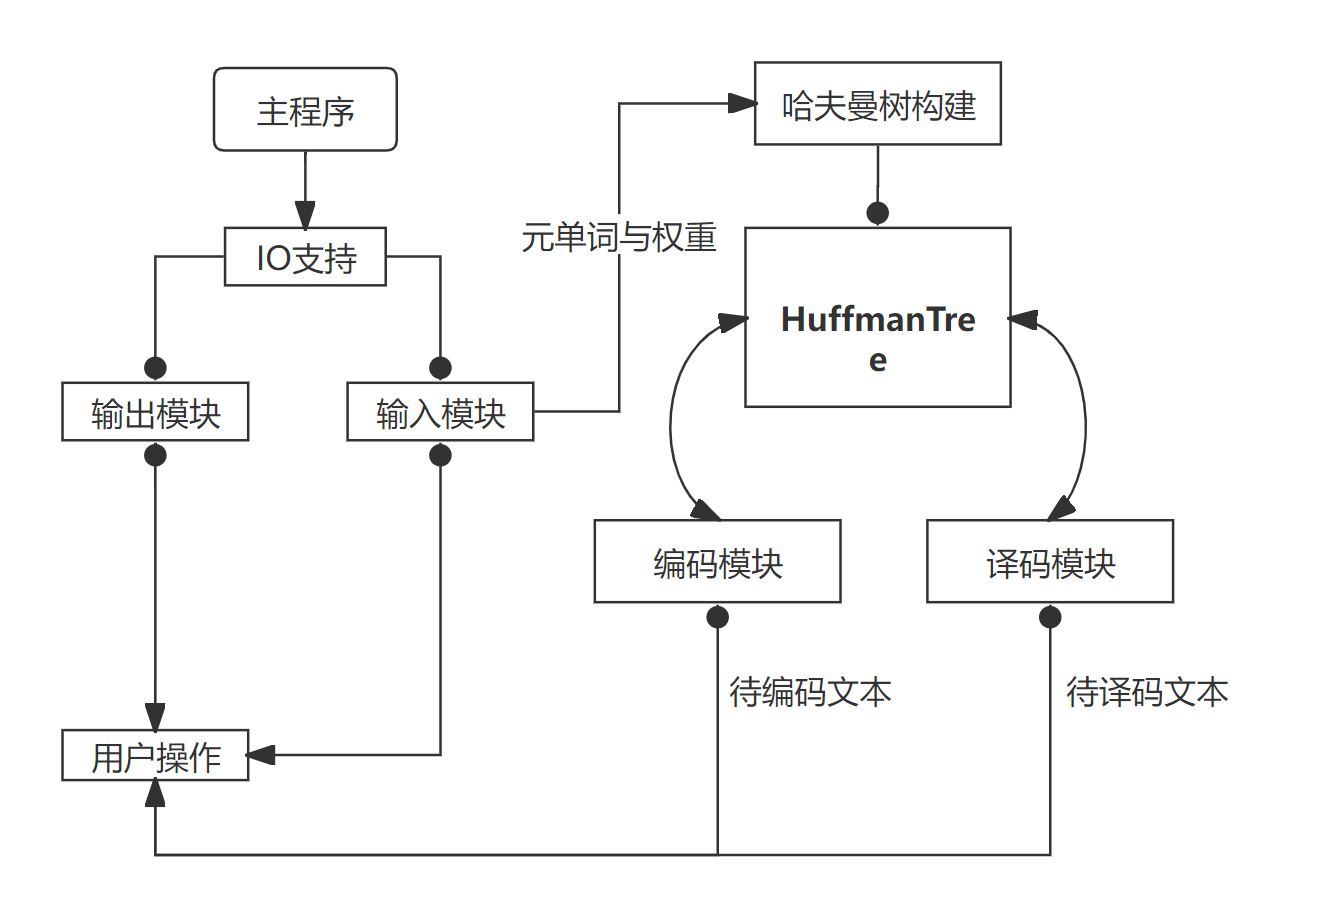
\includegraphics[width=125mm,height=85mm]{./assets/DS07-1}
	\end{minipage}
\end{figure}

\subsection*{三、详细设计}
\begin{algorithm}[H]
\begin{algorithmic}[1]
\caption{Construct Huffman Tree}
\Require Set of (word,weight) pairs: $\mathbf{I}$
\Ensure Huffman Tree of $\mathbf{I}$
\State let $\mathbf{S}$ $\leftarrow$ set of available Huffman Tree node
\For {item in $\mathbf{I}$}
	\State let item.left, item.right $\leftarrow$ nil
	\State $\mathbf{S}$.push(item)
\EndFor
\While {$\mathbf{S}$.size() > 2}
	\State let $\mathbf{node}$ $\leftarrow$ new Huffman Tree node
	\State pop the two terms with the largest weights from $\mathbf{S}$ as $\mathbf{node}$.left, $\mathbf{node}$.right
	\State $\mathbf{node}$.weight = $\mathbf{node}$.left.weight + $\mathbf{node}$.right.weight
	\State $\mathbf{S}$.push($\mathbf{node}$)
\EndWhile
\If {$\mathbf{S}$.size() = 2}
	\State let $\mathbf{root}$ $\leftarrow$ new Huffman Tree node
	\State $\mathbf{root}$.left = S[0], $\mathbf{root}$.right = S[1]
	\State return $\mathbf{root}$
\Else
	\State return $\mathbf{S}$[0]
\EndIf
\end{algorithmic}
\end{algorithm}

\begin{algorithm}[H]
\begin{algorithmic}[1]
\caption{Huffman Encode Single Word}
\Require HuffmanTree: $\mathbf{T}$, String: $\mathbf{word}$
\Ensure Encoded text of $\mathbf{word}$
\State let S $\leftarrow$ preorder tranverse sequence of $\mathbf{T}$
\State let $\mathbf{encoded}$ $\leftarrow$ new String
\For {node in S}
	\If {node.word = $\mathbf{word}$}
		\State return $\mathbf{encoded}$
	\EndIf
	\If {node is parent of previous node}
		\State encode.pop()
	\EndIf
	\If {node is left child of parent}
		\State $\mathbf{encoded}$.push("0")
	\Else
		\State $\mathbf{encoded}$.push("1")
	\EndIf
\EndFor
\State throw encode failure
\end{algorithmic}
\end{algorithm}

\begin{algorithm}[H]
\begin{algorithmic}[1]
\caption{Huffman Decode Single Word}
\Require HuffmanTree: $\mathbf{T}$, String: $\mathbf{encoded}$
\Ensure Decoded text of $\mathbf{encoded}$
\State let $\mathbf{node}$ $\leftarrow$ root of $\mathbf{T}$
\State let it $\leftarrow$ iterator of $\mathbf{encoded}$
\While {$\mathbf{node}$ is not a leaf node}
	\If {*it = "0"}
		\State $\mathbf{node}$ = $\mathbf{node}$.left
	\Else
		\State $\mathbf{node}$ = $\mathbf{node}$.right
	\EndIf
	\State it = next(it)
\EndWhile
\State return $\mathbf{node}$.word
\end{algorithmic}
\end{algorithm}

\subsection*{四、使用说明、测试分析与结果}
\subsubsection*{1、使用说明}
1) 本程序可以通过任意支持C++11及以上标准的编译器生成目标文件并在当前平台运行。 \par
2) 进入程序后务必依照需求的输入样式输入数据,手动输入与流式输入都是被允许的。 \par
3) 程序仅支持单字母编码。 \par
\subsubsection*{2、测试结果与分析}
2.1\;\textbf{实际环境} \par
对于所有输入,待编码字符为任意串,待解码字符为“0”“1”组成的任意串 \par
2.2\;\textbf{边界情况} \par
1) 待编解码串长度为0 \par
2) 待编码串存在未被哈夫曼树编码的单词 \par
3) 待译码串存在无法被哈夫曼树译码的“0”“1”串 \par
2.3\;\textbf{测试结果} \par
1) 目标正确输出空串 \par
2) 程序正常运行,但是编码结果混乱,无法正确编码 \par
3) 程序异常退出 \par
其中测试目标1)正常工作,代码设计初要求输入规范,故对于引起2)、3)问题的不规范输入,此处不做处理。 \par
关于具体原因: \par
对于2),编码算法建立在待编码单词在哈夫曼树中存在,故待编码字符为非法单词时,编码算法仅仅完成遍历并输出空串。 \par
对于3),译码算法假定待译码串正确且完整,当非法串输入时,译码算法无法保证子串对应的原码必然存在,其内部将存在越界访问字符串的行为,从而引发程序崩溃。 \par
\subsubsection*{3、调试过程问题分析与解决办法}
编码与测试环节皆未产生必须被处理的问题,跳过调试环节
\subsubsection*{4、设计与实现的回顾讨论与分析}
哈夫曼编码本质上是一个双射函数,而哈夫曼树就定义了该映射。代码的实现实质上就是三个部分: \par
1) 建立映射(建立哈夫曼树) \par
2) 描述正向映射(编码算法) \par
3) 描述逆向映射(译码算法) \par
哈夫曼树的理论描述很简单,但是在选择左右子树上并没有严格规定,因为交换顺序并不会改变建树过程的贪心策略保证的最短外部路径这一性质。在给出的代码中,其约定左子树的权重不小于右子树。 \par
关于编码,由于设计初并未给节点定义双亲域指针,故而最终算法的实现采取了遍历回溯+缓存的策略。在流程启动初,遍历的操作是耗时的,但该编码操作将随着程序的运行下降为哈希表查找的O(1)复杂度。 \par
关于译码算法,算法从根逐位向下寻找到叶子节点。对于哈夫曼这种变长编码,该算法普遍、高效且易于实现。 \par
\subsubsection*{5、运行界面}
\begin{figure}[H]
	\begin{minipage}[t]{\linewidth}
		\centering
		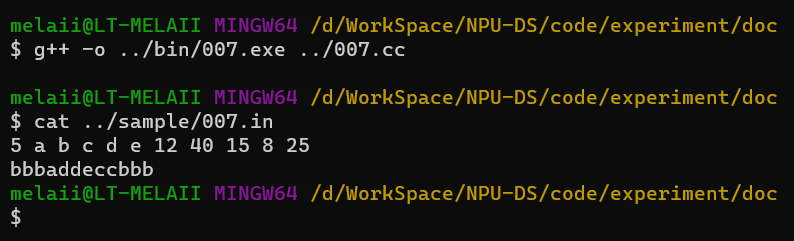
\includegraphics[width=125mm,height=40mm]{./assets/DS07-2}
		\caption{前置环境}
	\end{minipage}
\end{figure}
\begin{figure}[H]
	\begin{minipage}[t]{\linewidth}
		\centering
		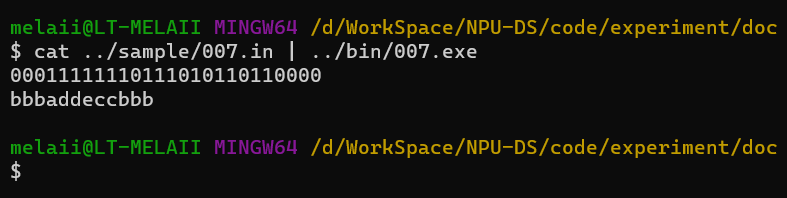
\includegraphics[width=125mm,height=36mm]{./assets/DS07-3}
		\caption{结果输出}
	\end{minipage}
\end{figure}

\subsection*{五、实验总结}
程序的逻辑整体上较为简单,主要的时间花费在了程序结构设计的选择上。哈夫曼树在简单的定义下满足了其最短外部路径的性质,但是并未对具体过程有唯一确定的算法描述。而这一模糊不定的部分可能成为一个阻碍,也可以成为改进与自由发挥的点。按部就班地按照参考算法实验固然是不错的,但是另辟蹊径或是尝试改造才有加深理解甚至是突破的潜力。曾经并非没有接触过哈夫曼编码,但是本次实验却是我实打实的一次完整实现,也算是在某条不知名的道路上留下了一个新的脚印。

~\\
\zihao{-4}
\textbf{教师评语:}
~\\
\textbf{实验成绩:}

\begin{flushright}
\mbox{指导教师签名:\qquad\qquad} \\
\mbox{批阅日期:\qquad\qquad}
\end{flushright}

\end{document}